% !TEX program = lualatex
% !TEX encoding = UTF-8 Unicode
% !TEX spellcheck = en
% spell-checker:ignore RWTH, leavevmode, qedhere, siunitx, titlehead
\documentclass[fleqn,bibliography=totoc,index=totoc,paper=A4,twoside=semi,DIV=12]{scrbook}
\usepackage[american]{babel}
\usepackage[T1]{fontenc}
\usepackage[utf8]{inputenc}
% spell-checker:disable
% Restore the typical KOMA-Script style fonts, which are changed by setting fontenc to T1
\usepackage{lmodern}
\DeclareSymbolFont{largesymbols}{OMX}{cmex}{m}{n} % use cmex rather than lmex
% spell-checker:enable
% \usepackage{stmaryrd} 
\usepackage{styleBB}
\usepackage{bm} 
% \usepackage{xltxtra}  
\usepackage{multirow}
\usepackage{algorithm2e}
\usepackage{nicefrac}
\usepackage{afterpage}
\usepackage{graphicx}
\usepackage{caption}
\usepackage{subcaption}
\usetikzlibrary{positioning}
% \usepackage[symbols,nogroupskip,sort=none]{glossaries-extra}
\usepackage[symbols,nogroupskip,nonumberlist,sort=use]{glossaries-extra}
\makenoidxglossaries
\usepackage[utf8]{inputenc}
\usepackage{pgfplots}
% \DeclareUnicodeCharacter{2212}{−}
\usepgfplotslibrary{groupplots,dateplot}
\usetikzlibrary{patterns,shapes.arrows}
\pgfplotsset{compat=newest}
\usepackage{stmaryrd}
\SetSymbolFont{stmry}{bold}{U}{stmry}{m}{n}
% \SetSymbolFont{stmry}{bold}{U}{stmry}{b}{n}
% \SetSymbolFont{stmry}{bold}{U}{stmry}{b}{n}
% \usepackage{stmaryrd}
% \SetSymbolFont{stmry}{bold}{U}{stmry}{m}{n}
% \usepackage[acronym]{glossaries}
% \usepackage{algorithm}
% \usepackage{algpseudocode}
% \usepackage{algorithmic}
\usepackage{silence}
% \WarningFilter{latex}{Marginpar on page}

\setlength{\marginparwidth}{2cm}
\usepackage[textsize=tiny]{todonotes}

\graphicspath{
{./figures/},
}

\pgfplotsset{
  table/search path={data},
}
% \usepackage{biblatex}
\addbibresource{/Users/rknot/sciebo/jabref_files/database.bib}

\renewcommand{\chaptermark}[1]{\markboth{\thechapter\,\,#1}{}}
\renewcommand{\sectionmark}[1]{\markright{\thesection\,\,#1}}
\newtheorem{problem}{Problem}
% \newcommand{\vct}[1]{\bm{#1}}
\usepackage[headsepline]{scrlayer-scrpage}
\clearpairofpagestyles
\addtokomafont{pagehead}{\normalfont\bfseries}
\lohead{\rightmark}
\rohead{\thepage}
\lehead{\thepage}
\rehead{\leftmark}

\makeindex

% Useful to build the dvi/pdf without any images
%\renewcommand{\includegraphics}[2][a]{image}
% Useful to let jpg be preferred to png by \includegraphics (default behavior is the other way round) if no suffix is specified.
%\DeclareGraphicsExtensions{.pdf,.jpg,.png}




\includeonly{
            %  00.frontmatter,
            %  dedication,
            %  abstract,
            %  acknowledgements,
             symbols,
             00,
             01,
             02,
            %  03,
            %  04,
            %  05,
             06,
             }


\begin{document}

% Get rid of the double spacing at the end of a sentence.
\frenchspacing
% Configure the "depth" of the table of contents
\setcounter{tocdepth}{2}
% Change the numbering of the first enumerated list to (i)
\renewcommand{\labelenumi}{(\roman{enumi})}
% Change the numbering of the second enumerated list to (1)
\renewcommand{\labelenumii}{(\arabic{enumii})}

\titlehead{%
\raggedleft
\includegraphics[scale=0.65]{./figures/rwth_aices_cmyk-crop.pdf}\\[1ex]
\centering
The present work was submitted to the\\Aachen Institute for Advanced Study in Computational Engineering Science\\
   RWTH Aachen University\\
   Junior Professorship of Mathematical Image and Signal Processing
}\subject{Master's thesis}
\title{Deep Unfolding of Wirtinger Flow Type Schemes}
\author{Ali Darijani}
\date{\today}
\publishers{
\begin{tabular}{rl}
% 1\textsuperscript{st} supervisor:&Professor Benjamin Berkels\\
supervisor:&Professor Benjamin Berkels\\
% 2\textsuperscript{nd} supervisor:&Professor Jane Q. Public
\end{tabular}
}

% \lowertitleback{typeset using {\KOMAScript} and {\LaTeX}}
\lowertitleback{Typesetted using {\TeX}, {\AmS-\TeX}, and {\KOMAScript}\\Happy \TeX-ing!}


\frontmatter

\maketitle 

\tableofcontents

\mainmatter

\chapter*{}
\addcontentsline{toc}{chapter}{Dedication}  



% \clearpage
\begin{center}
    \thispagestyle{empty}
    \vspace*{\fill}
    \large TO THE MEMORY OF THE MOHAMMAD MAHDI ELYASI\\
    A DOWN TO EARTH TRtUE PHYSICIST AND A LEGENDARY PETROLHEAD
    \vspace*{\fill}
\end{center}
% \clearpage

\endinput
\chapter*{Abstract}
\addcontentsline{toc}{chapter}{Abstract}  

Physical measurements in settings where light, electrons, and similar existences are involved will result in a phase loss in the
mathematical formulation. The phenomenon is called \emph{Phase Problem} and the methods developed to tackle the said unpleasantness
are called \emph{Phase Retrieval} methods. Due to its presence in a wide spectrum of applications ranging from X-ray crystallography, 
transmission electron microscopy to quantum mechanics, the retrieval methods are highly investigated and coveted. One of the contemporary 
breakthroughs are the \emph{\ac{WF}} variants which are nice and relatively easy algorithms with small memory footprints equipped with nice 
guarantees on the solutions. \ac{WF} variants are derived from minimizing a certain functional and are of iterative nature. Like most 
iterative approaches they are certain parameters that need to be fixed that greatly influence the convergence rate and stability. We aimed 
to optimized these parameters using \emph{Deep Unfolding} which is an emerging technic from the data-driven side of approaches. Deep Unfolding 
is basically unfolding an iterative algorithm finite times and putting it into a neural network to be trained. Anyone who has been exposed 
to machine learning would realize that \emph{Hyperparameter} optimization must be done to close the study which is what we did.       


\endinput
\chapter*{Acknowledgements}
\addcontentsline{toc}{chapter}{Acknowledgements}


I would like to thank:\\\\
\noindent Fatemeh Darijani, Nabiollah Darijani, Razmkhah Darijani, Yadollah Darijani, Eve Darijani, Hossein Darijani, 
Kaiser Darijani, Shahnesa Darijani, Fatemeh Darijani, Abdullah Darijani, Rasul Darijani, Samira Darijani, 
Mohammad Reza Haghighi, Mahmoud Nasiri, Sedigheh Darijani, Masoud Jafari, Hossein Darijani, Hassan Sedigh, 
Atefeh Hasanzadeh, Siavash Mirshams Shahshahani, Masoud Aghasi, Mir Abbas Jalali, Donald Theodore Greenwood, Elnaz Naghibi, 
Singiresu S. Rao, Elahe Alizadeh, Famida Fallah, Egor Pavlovich Popov, Stepan Prokopovich Timoshenko, GholamHossein Farrahi, 
Mahsa Ghasemi, Samaneh Sadri, Mohammad Mahdi Elyasi, Ghazal Esmaeili, Navid Gharavi, Yahya Kabiri Renani, Katsuhiko Ogata, 
Mohammad Behshad Shafii, Amirreza Gandomkar, Frank P. Incropera, Hassan Zohoor, Melika Shahhosseini, Ali Mousavi, 
Saeed Rezaei, Negar Nabatian, Mohamad Taghi Ahmadian, Afsaneh Rahmani, Ayatollah Darijani, Shahnaz Darijani, 
Hassan Sedigh, Ali Darijani, Mohammad Darijani, Morteza Mohammadi, Mahsa Barzegar Keshteli, Siamak Sheykhha, Amin Rahmati, 
Omid Zarei, Mahsa Fatehi, Manuel Torrilhon, Hossein Gorji, Mohsen Sadr, Reza Ghaffari, CATS IT, Christoph Stolz, 
Christian Delzepich, Léon Benthaus, Zahra Sadat Hajseyed Nasrollah, Marcus Stoffel, Nima Shirafkan, Nadia Amira, 
Roger A. Sauer, Natalia Tager, Mikhail Itskov, Gerhard Alfred Holzapfel, Yavuz Ba\c{s}ar, Dieter Weichert, 
Farzad Shirazian, Behzad Zargar, Paolo Bientinesi, Marek Behr, Maximilian Schuster, Georg May, Nick Trefethen, 
David Bau {\MakeUppercase{\romannumeral 3}}, James Weldon Demmel Jr., Yousef Saad, Benjamin Berkels, Sven Gro{\ss}, 
Arnold Reusken, Adel Mhamdi, Lutz Angermann, Peter Knabner, Randall J. LeVeque, Wolfgang Hackbusch, John Burkardt, 
Ilinca Burdulea, Alexander Fleming, Abhinav Jha,  Tuan Vo, Holger Rauhut, Bastian Leibe, Martin Grohe, 
Christopher Michael Bishop, Ian Goodfellow, Yoshua Bengio, Aaron Courville, Bahram Ashrafi, Maryam Sodagar, 
Alireza Khoshhal, Maryam Hassani, Kristian Bredies, Dirk Lorenz, Serge Lang, Emanuel Carneiro, Hans Wilhelm Alt, 
Elias Menachem Stein, Rami Shakarchi, Terence Tao, Walter Rudin, Nicholas Higham, Steven George Krantz, RWTH IT, 
Farzad Shirazian, Shadi Shirazian, Zahra Sadat Hajseyed Nasrollah, and Benjamin Berkels,\\\\
for what I am today. The list is mostly chronologically ordered and the inclusion reason can almost be anything. 
As I do not have such a great memory many names are lost inevitably and I am deeply saddened by this and yet still 
grateful to the unsung heroes  and forever in their debt.
\\\\
-ad\\
Aachen, Germany\\

\endinput 
\glsxtrnewsymbol[description={inclusion signs}]{inclusion signs}{\ensuremath{\subset,\supset}}
\glsxtrnewsymbol[description={rational field}]{rational field}{\ensuremath{\mathbb{Q}}}
\glsxtrnewsymbol[description={least upper bound}]{least upper bound}{\ensuremath{\sup}}
\glsxtrnewsymbol[description={greatest lower bound}]{greatest lower bound}{\ensuremath{\inf}}

\glsxtrnewsymbol[description={null vector}]{null vector}{\ensuremath{\boldsymbol{0}}}
\glsxtrnewsymbol[description={inner product}]{inner product}{\ensuremath{\boldsymbol{x} \cdot \boldsymbol{y}}}
\glsxtrnewsymbol[description={elementwise absolute value of a multidimensional array $\boldsymbol{X}$} in the vector space $X$]{elementwise abs}{\ensuremath{\left| \boldsymbol{X}\right|_{e_X} }}\index{Product!Elementwise}
\glsxtrnewsymbol[description={elementwise/Hadamard product between two multidimensional array $\boldsymbol{X},\boldsymbol{Y}$}]{elementwise prod}{\ensuremath{\boldsymbol{X}\odot\boldsymbol{Y}}}\index{Product!Hadamard}
\glsxtrnewsymbol[description={sequence}]{sequence}{\ensuremath{\{x_n\}}}
\glsxtrnewsymbol[description={union}]{union}{\ensuremath{\bigcup,\cup}}
\glsxtrnewsymbol[description={intersection}]{intersection}{\ensuremath{\bigcap,\cap}}
\glsxtrnewsymbol[description={segment}]{segment}{\ensuremath{\left(a,b\right)}}
\glsxtrnewsymbol[description={interval}]{interval}{\ensuremath{\left[a,b\right]}}
\glsxtrnewsymbol[description={half intervals}]{half intervals}{\ensuremath{\left(a,b\right],\left[a,b\right)}}
\glsxtrnewsymbol[description={complement of $E$}]{complement of E}{\ensuremath{E^\mathsf{c}}}
\glsxtrnewsymbol[description={limit points of $E$}]{limit points of E}{\ensuremath{E^{'}}}
\glsxtrnewsymbol[description={closure of $E$}]{closure of E}{\ensuremath{\overline{E}}}
\glsxtrnewsymbol[description={limit}]{limit}{\ensuremath{\lim}}
\glsxtrnewsymbol[description={converges to}]{converges to}{\ensuremath{\to}}
\glsxtrnewsymbol[description={lim sup}]{lim sup}{\ensuremath{\lim \sup}}
\glsxtrnewsymbol[description={lim inf}]{lim inf}{\ensuremath{\lim \inf}}
\glsxtrnewsymbol[description={composition}]{composition}{\ensuremath{g \circ f}}
\glsxtrnewsymbol[description={right-hand limit}]{right-hand limit}{\ensuremath{f(x+)}}
\glsxtrnewsymbol[description={left-hand limit}]{left-hand limit}{\ensuremath{f(x-)}}
\glsxtrnewsymbol[description={derivatives}]{derivatives}{\ensuremath{f^{\prime}, \boldsymbol{f}(\boldsymbol{x})^{\prime}}}
\glsxtrnewsymbol[description={Riemann sums}]{Riemann sums}{\ensuremath{U(\boldsymbol{P},f),U(\boldsymbol{P},f,\alpha),L(\boldsymbol{P},f),L(\boldsymbol{P},f,\alpha)}}
\glsxtrnewsymbol[description={classes of Riemann (Stieltjes) integrable functionas}]{classes of Riemann (Stieltjes) integrable functionas}{\ensuremath{\mathcal{R},\mathcal{R}(\alpha)}}
\glsxtrnewsymbol[description={space of continiuous functions}]{space of continiuous functions}{\ensuremath{\mathcal{C}(X)}}
\glsxtrnewsymbol[description={norm}]{norm}{\ensuremath{\left|\left|\;\;\right|\right|}}
\glsxtrnewsymbol[description={exponential function}]{exponential function}{\ensuremath{\exp}}
\glsxtrnewsymbol[description={Dirichlet kernel}]{Dirichlet kernel}{\ensuremath{D_N}}
\glsxtrnewsymbol[description={gamma function}]{gamma function}{\ensuremath{\Gamma(x)}}

\glsxtrnewsymbol[description={spaces of linear transformation}]{spaces of linear transformation}{\ensuremath{L(X),L(X,Y)}}
\glsxtrnewsymbol[description={matrix}]{matrix}{\ensuremath{\left[\boldsymbol{A}\right]}}
\glsxtrnewsymbol[description={partial derivative}]{partial derivative}{\ensuremath{D_Jf}}
\glsxtrnewsymbol[description={gradient}]{gradient}{\ensuremath{\nabla f}}
\glsxtrnewsymbol[description={classes of differentiable functions}]{classes of differentiable functions}{\ensuremath{\mathcal{C}^\prime,\mathcal{C}^{\prime\prime}}}
\glsxtrnewsymbol[description={determinant}]{determinant}{\ensuremath{\det \left[\boldsymbol{A}\right]}}
\glsxtrnewsymbol[description={Jacobian}]{Jacobian_implicit}{\ensuremath{\boldsymbol{J}_f(\boldsymbol{x})}}
\glsxtrnewsymbol[description={Jacobian}]{Jacobian_explicit}{\ensuremath{\frac{\partial(y_1,\cdots,y_n)}{\partial(x_1,\cdots,x_n)}}}
\glsxtrnewsymbol[description={$k$-cell}]{k-cell}{\ensuremath{\mathbb{I}^k}}
\glsxtrnewsymbol[description={$k$-simplex}]{k-simplex}{\ensuremath{\mathbb{Q}^k}}
\glsxtrnewsymbol[description={basic $k$-form}]{basic k-form}{\ensuremath{d\boldsymbol{x}_{\boldsymbol{I}}}}
\glsxtrnewsymbol[description={multiplication symbol}]{multiplication symbol}{\ensuremath{^\wedge}}

\glsxtrnewsymbol[description={transform of $\omega$}]{transform of omega}{\ensuremath{\omega_{\boldsymbol{T}}}}
\glsxtrnewsymbol[description={boundary operator}]{boundary operator}{\ensuremath{\partial}}
\glsxtrnewsymbol[description={curl}]{curl}{\ensuremath{\nabla \times \boldsymbol{F}}}
\glsxtrnewsymbol[description={divergence}]{divergence}{\ensuremath{\nabla\cdot\boldsymbol{F}}}
\glsxtrnewsymbol[description={ring of elementary sets}]{ring of elementary sets}{\ensuremath{\mathcal{E}}}
\glsxtrnewsymbol[description={Lebesgue measure}]{Lebesgue measure}{\ensuremath{m}}
\glsxtrnewsymbol[description={measure}]{measure}{\ensuremath{\mu}}
\glsxtrnewsymbol[description={families of measurable sets}]{families of measurable sets}{\ensuremath{\mathcal{M}_F,\mathcal{M}}}
\glsxtrnewsymbol[description={positive(negative) part of $f$}]{posotove(negative) part of $f$}{\ensuremath{f^+,f^-}}
\glsxtrnewsymbol[description={characteristic function}]{characteristic function}{\ensuremath{K_{E}}}
\glsxtrnewsymbol[description={classes of Lebesgue-integrable functions}]{classes of Lebesgue-integrable functions}{\ensuremath{\mathcal{L},\mathcal{L}(\mu),\mathcal{L}^2,\mathcal{L}^2(\mu)}}


%%%%%%%%%%%%%%%%%%%%%%%%%%%%%%%%%%%%%%%%%%%%%%%%%%%%%%%%%%%%%%%%%%%%%%%%%%%%%%%%%%%%%%%%%%%%%%%%%%%%%%%%%%%%%%%%%%%%%%%
%%%%%%%%%%%%%%%%%%%%%%%%%%%%%%%%%%%%%%%%%%%%%%%%%%%%%%%%%%%%%%%%%%%%%%%%%%%%%%%%%%%%%%%%%%%%%%%%%%%%%%%%%%%%%%%%%%%%%%%
%%%%%%%%%%%%%%%%%%%%%%%%%%%%%%%%%%%%%%%%%%%%%%%%%%% Used Symbols %%%%%%%%%%%%%%%%%%%%%%%%%%%%%%%%%%%%%%%%%%%%%%%%%%%%%%
%%%%%%%%%%%%%%%%%%%%%%%%%%%%%%%%%%%%%%%%%%%%%%%%%%%%%%%%%%%%%%%%%%%%%%%%%%%%%%%%%%%%%%%%%%%%%%%%%%%%%%%%%%%%%%%%%%%%%%%
%%%%%%%%%%%%%%%%%%%%%%%%%%%%%%%%%%%%%%%%%%%%%%%%%%%%%%%%%%%%%%%%%%%%%%%%%%%%%%%%%%%%%%%%%%%%%%%%%%%%%%%%%%%%%%%%%%%%%%%
\glsxtrnewsymbol[description={inequality signs}]{inequality signs}{\ensuremath{<,\leq,>,\geq}}
\glsxtrnewsymbol[description={belongs to}]{in}{\ensuremath{\in}}  
\glsxtrnewsymbol[description={does not belong to}]{not in}{\ensuremath{\notin}}
\glsxtrnewsymbol[description={scalar product on the vector space $X$}]{scalar product}{\ensuremath{\left( \boldsymbol{\cdot} , \boldsymbol{\cdot} \right)_X}}
\glsxtrnewsymbol[description={the norm induced by the scalar product on the vector space $X$}]{induced norm}{\ensuremath{\left| \boldsymbol{\cdot} \right|_X}}
\glsxtrnewsymbol[description={absolute value/element-wise absolute value}]{absolute value/element-wise absolute value}{\ensuremath{\left| z \right|}}
\glsxtrnewsymbol[description={exponential}]{exponential}{\ensuremath{\exp}} 
\glsxtrnewsymbol[description={summation over $i$}]{summation over $i$}{\ensuremath{\sum_{i=p}^{i=q}a(i)}}



\glsxtrnewsymbol[description={real field}]{real field}{\ensuremath{\mathbb{R}}}
\glsxtrnewsymbol[description={complex field}]{complex field}{\ensuremath{\mathbb{C}}}
\glsxtrnewsymbol[description={euclidean $d$-space}]{euclidean $d$-space}{\ensuremath{\mathbb{R}^d}}
\glsxtrnewsymbol[description={complex $d$-space}]{complex $d$-space}{\ensuremath{\mathbb{C}^d}}

\glsxtrnewsymbol[description={infinities}]{infinities}{\ensuremath{+\infty,-\infty,\infty}}


\glsxtrnewsymbol[description={operator $\boldsymbol{A}$}]{operator A}{\ensuremath{\boldsymbol{A}}}
\glsxtrnewsymbol[description={adjoint operator of the operator $\boldsymbol{A}$}]{adjoint operator of the operator A}{\ensuremath{\boldsymbol{A}^*}}
\glsxtrnewsymbol[description={complex conjugate}]{complex conjugate}{\ensuremath{\overline{z}}}
\glsxtrnewsymbol[description={real part}]{real part}{\ensuremath{\operatorname{Re}(z)}}
\glsxtrnewsymbol[description={imaginary part}]{imaginary part}{\ensuremath{\operatorname{Im}(z)}}
\glsxtrnewsymbol[description={summation sign}]{summation sign}{\ensuremath{\sum}}

\glsxtrnewsymbol[description={standard cartesian basis}]{standard cartesian basis}{\ensuremath{\{\boldsymbol{e}_1,\cdots,\boldsymbol{e}_n\}}}
\glsxtrnewsymbol[description={general $1$-$d$ basis}]{general $1$-$d$ basis}{\ensuremath{\{\boldsymbol{g}^1,\cdots,\boldsymbol{g}^n\}}}
\glsxtrnewsymbol[description={general $2$-$d$ basis}]{general $2$-$d$ basis}{\ensuremath{\left\{\boldsymbol{g}^{i,j}\right\}_{\substack{i=1,\ldots,m\\ j=1,\ldots,n}}}}
\glsxtrnewsymbol[description={differentiation operator}]{differentiation operator}{\ensuremath{\mathrm{d}}}
% \glsxtrnewsymbol[description={differentiation operator multidimensional for }]{differentiation operator multidimensional}{\ensuremath{\mathrm{d}}}

\chapter{Mathematical Preliminaries}






\begin{Def}\label{def:1ddft}
    \emph{$1$D Discrete Fourier Transform}\\
    The \emph{$1$D Discrete Fourier Transform} of the $1$D array $\boldsymbol{X} \in \mathbb{C}^{N}$ is denoted by 
    $\hat {\boldsymbol{X}} \in \mathbb{C}^{N}$ and is defined by
    \begin{equation}\label{eq:1ddft}
        \{\hat {\boldsymbol{X}}\}_{k} \coloneqq \frac{1}{N}\sum_{n=0}^{N-1} \{{\boldsymbol{X}}\}_{n}\exp\left({\frac{-2\pi ink}{N}}\right)
    \end{equation}
    and to get back the original array one can use the inversion formula
    \begin{equation}\label{eq:1didft}
        \{{\boldsymbol{X}}\}_{n} \coloneqq \sum_{k=0}^{N-1}\{\hat {\boldsymbol{X}}\}_{k}\exp\left({\frac{2\pi ink}{N}}\right)
    \end{equation}    
\end{Def}

As it is evident from the formula the $1$D Discrete Fourier Transform is a linear transformation therefor 
there a corresponding matrix and basis vectors. The matrix is dense matrix and due to computational efficiency 
is almost never computed directly, however taking a closer look at the basis vectors would shed some light on 
the nature of the said transform and is a time well spent.

\begin{Prop}
    For complex valued vectors $\boldsymbol{x},\boldsymbol{y} \in \mathbb{C}^n$ the following is a proper scalar product
    \begin{equation*}
        \boldsymbol{x} = \left\{x_i\right\}_{i=1,\ldots,n-1}, \quad \boldsymbol{y} = \left\{y_i\right\}_{i=1,\ldots,n-1}
    \end{equation*}
    \begin{equation*}
        \langle\boldsymbol{x},\boldsymbol{y}\rangle \coloneqq \sum_{i=0}^{n-1} x_i \overline{y_i} 
    \end{equation*}
\end{Prop}

\begin{proof}
    You can consult \cite{wavelets_linear_algebra_frazier} or \cite{matrix_analysis_horn} \cite{numerical_tensor_hackbusch}.
\end{proof}






\begin{Prop}\label{Prop:1ddftbasisvectors}
    The basis vectors
    \begin{equation}\label{eq:1ddftbasisvectors}
        \boldsymbol{g}^n = \left\{\exp\left({\frac{-2\pi ink}{N}}\right)\right\}_{k=0,\ldots,N-1}
    \end{equation}
    are orthogonal to each other with respect to the usual inner product for complex valued vectors 
    with the normalization constant of $N$
    \begin{equation}
        \langle\boldsymbol{g}^n,\boldsymbol{g}^{n'}\rangle= N \delta_{n,n'}
    \end{equation}
\end{Prop}

\begin{proof}
    \begin{equation*}
        \boldsymbol{g}^n = \left\{\exp\left({\frac{-2\pi ink}{N}}\right)\right\}_{k=0,\ldots,N-1}, \quad \boldsymbol{g}^{n'} = \left\{\exp\left({\frac{-2\pi in'k}{N}}\right)\right\}_{k=0,\ldots,N-1}
    \end{equation*}
    \begin{equation*}
    \begin{split} 
        \langle\boldsymbol{g}^n,\boldsymbol{g}^{n'}\rangle &= \sum_{k=0}^{N-1} \exp\left({\frac{-2\pi ink}{N}}\right)\overline{\exp\left({\frac{-2\pi in'k}{N}}\right)}
        = \sum_{k=0}^{N-1} \exp\left({\frac{-2\pi ink}{N}}\right)\exp\left({\frac{+2\pi in'k}{N}}\right)\\
        &= \sum_{k=0}^{N-1} \exp\left({\frac{-2\pi i(n'-n)k}{N}}\right)=
        \begin{cases}
            N & \text{when $n = n'$}\text{(trivial)},\\
            0 & \text{when $n\neq n'$}\text{(using geometric sum formula)}.
        \end{cases}
    \end{split}
\end{equation*}
    
\end{proof}


\begin{Rem}
    showing the Fourier transform by a matrix \cite{wavelets_linear_algebra_frazier} \cite{image_processing_bredies} \cite{signal_miller}.
    Let $W_N$ be the matrix with $\left\{W_N\right\}_{\substack{mn \\ 0 \leq m,n \leq N-1}}$ 
    \begin{equation*}
        W_N \coloneqq 
        \begin{bmatrix}
            1     & 1                & 1                   & 1                   & \cdots & 1                      \\
            1     & \omega_{N}^{}    & \omega_{N}^{2}      & \omega_{N}^{3}      & \cdots & \omega_{N}^{N-1}       \\
            1     & \omega_{N}^{2}   & \omega_{N}^{4}      & \omega_{N}^{6}      & \cdots & \omega_{N}^{2(N-1)}    \\
            1     & \omega_{N}^{3}   & \omega_{N}^{6}      & \omega_{N}^{9}      & \cdots & \omega_{N}^{3(N-1)}    \\
            \cdot & \cdot            & \cdot               & \cdot               & \cdots & \cdot                  \\ 
            \cdot & \cdot            & \cdot               & \cdot               & \cdots & \cdot                  \\ 
            1     & \omega_{N}^{N-1} & \omega_{N}^{2(N-1)} & \omega_{N}^{3(N-1)} & \cdots & \omega_{N}^{(N-1)(N-1)}
            \end{bmatrix}
    \end{equation*}
    where $\omega_N = e^{-2\pi i/N}$ then $e^{-2\pi i/N} = \omega_N^{mn}$
\end{Rem}








\begin{Def}\label{def:2ddft}
    \emph{$2$D Discrete Fourier Transform}\\
    The \emph{$2$D Discrete Fourier Transform} of the $2$D array $\boldsymbol{X} \in \mathbb{C}^{N \times M}$ is denoted by 
    $\hat {\boldsymbol{X}} \in \mathbb{C}^{N \times M}$ and is defined by
    \begin{equation}\label{eq:2ddft}
        \{\hat {\boldsymbol{X}}\}_{k,l} \coloneqq \frac{1}{MN}\sum_{m=0}^{M-1}\sum_{n=0}^{N-1} \{{\boldsymbol{X}}\}_{n,m}\exp\left({\frac{-2\pi ink}{N}}\right)\exp\left({\frac{-2\pi iml}{M}}\right)
    \end{equation}
    and to get back the original array one can use the inversion formula
    \begin{equation}\label{eq:2didft}
        \{{\boldsymbol{X}}\}_{n,m} \coloneqq \sum_{k=0}^{N-1}\sum_{l=0}^{M-1}\{\hat {\boldsymbol{X}}\}_{k,l}\exp\left({\frac{2\pi ink}{N}}\right)\exp\left({\frac{2\pi iml}{M}}\right)
    \end{equation}    
\end{Def}

As it is evident from the formula the $2$D Discrete Fourier Transform is a linear transformation therefor 
there a corresponding matrix and basis vectors. The matrix is dense matrix and due to computational efficiency 
is almost never computed directly, however taking a closer look at the basis vectors would shed some light on 
the nature of the said transform and is a time well spent.



\begin{Prop}
    For complex valued second order tensors $\boldsymbol{X},\boldsymbol{Y} \in \mathbb{C}^{m \times n}$ the following is a proper scalar product
    \begin{equation*}
        \boldsymbol{X} = \left\{X_{i,j}\right\}_{\substack{i=0,\ldots,m-1\\ j=0,\ldots,n-1}}, \quad \boldsymbol{Y} = \left\{Y_{i,j}\right\}_{\substack{i=0,\ldots,m-1\\ j=0,\ldots,n-1}}
    \end{equation*}
    \begin{equation*}
        \langle\boldsymbol{X},\boldsymbol{Y}\rangle \coloneqq \sum_{j=0}^{n-1}\sum_{i=0}^{m-1} X_{i,j} \overline{Y_{i,j}} 
    \end{equation*}
\end{Prop}

Which is also called 

\begin{proof}
    You can consult \cite{wavelets_linear_algebra_frazier} or \cite{matrix_analysis_horn} \cite{numerical_tensor_hackbusch}
\end{proof}

\begin{Prop}\label{Prop:2ddftbasisvectors}
    The basis vectors
    \begin{equation}\label{eq:2ddftbasisvectors}
        \boldsymbol{g}^{n,m} = \left\{\exp\left({\frac{-2\pi ink}{N}}\right)\exp\left({\frac{-2\pi iml}{M}}\right)\right\}_{\substack{k=0,\ldots,N-1\\l=0,\ldots,M-1}}
    \end{equation}
    are orthogonal to each other with respect to the usual inner product for complex valued vectors 
    with the normalization constant of $MN$
    \begin{equation}
        \langle\boldsymbol{g}^{n,m},\boldsymbol{g}^{n',m'}\rangle= MN \delta_{n,n'}\delta_{m,m'}
    \end{equation}
\end{Prop}

\begin{proof}
    \begin{align*} 
        \boldsymbol{g}^{n,m}    &= \left\{\exp\left({\frac{-2\pi ink}{N}}\right)\exp\left({\frac{-2\pi iml}{M}}\right)\right\}_{\substack{k=0,\ldots,N-1\\l=0,\ldots,M-1}}\\
        \boldsymbol{g}^{n',m'}  &= \left\{\exp\left({\frac{-2\pi in'k}{N}}\right)\exp\left({\frac{-2\pi im'l}{M}}\right)\right\}_{\substack{k=0,\ldots,N-1\\l=0,\ldots,M-1}}
    \end{align*}
    \begin{equation*}
        \begin{split}  
            \langle\boldsymbol{g}^{n,m},\boldsymbol{g}^{n',m'}\rangle &= \sum_{l=0}^{M-1}\sum_{k=0}^{N-1} \exp\left({\frac{-2\pi ink}{N}}\right)\exp\left({\frac{-2\pi iml}{M}}\right)\overline{\exp\left({\frac{-2\pi in'k}{N}}\right)\exp\left({\frac{-2\pi im'l}{M}}\right)}\\
            &= \sum_{l=0}^{M-1}\sum_{k=0}^{N-1} \exp\left({\frac{-2\pi ink}{N}}\right)\exp\left({\frac{-2\pi iml}{M}}\right)\exp\left({\frac{+2\pi in'k}{N}}\right)\exp\left({\frac{+2\pi im'l}{M}}\right)\\
            &= \sum_{l=0}^{M-1}\sum_{k=0}^{N-1} \exp\left({\frac{-2\pi i(n'-n)k}{N}}\right)\exp\left({\frac{-2\pi i(m'-m)l}{M}}\right)\\
            &= \sum_{k=0}^{N-1} \exp\left({\frac{-2\pi i(n'-n)k}{N}}\right)\sum_{l=0}^{M-1} \exp\left({\frac{-2\pi i(m'-m)k}{M}}\right)\\
            &= 
            \begin{cases}
                MN & \text{when $n = n' \wedge m=m'$}\text{(trivial)},\\
                0 & \text{when $\neg(n = n' \wedge m=m')$}\text{(using geometric sum formula)}.
            \end{cases}    
        \end{split}
    \end{equation*}
    

    
\end{proof}



Fast Fourier Transform \cite{fft_cooley_tukey} \cite{fft_good_pfa} \cite{wavelets_linear_algebra_frazier} \cite{algorithm_clrs}




\begin{Thm}\label{theorem:dft is unitary}
    
    Here goes the actual theorem description.
\end{Thm}







  
\include{01}
\chapter{Wirtinger Flow}

The whole thing about \emph{Wirtinger Flow} variants started with the seminal work of Candes and Soltanolkotabi\cite{bib:wf}.
The most important improvements chronologically were done by Candes and Chen\cite{bib:twf}, Kolte and Özgür\cite{bib:itwf}, and Zhang et al.\cite{bib:rfw-irwf}.
For a quite extensive survey on \emph{Wirtinger Flow} variants please refer to Liu et al.\cite{bib:wf-survey}. Chandra et al.\cite{bib:phasepack} 
gathered quite number of \emph{Phase Retrieval} methods including a couple of \emph{Wirtinger Flow} variants in the MATLAB\textregistered\space 
problem solving environment in a uniform manner.\\
We quickly go over the problem formulation, difficulties, algorithms, and at the of the chapter we give some numerical experiments we are going
to refer to in the subsequent chapters.

\section{Problem Formulation}
Consider the ray $\boldsymbol{x} \in \mathbb{C}^{n \times 1}$ is emitted onto the object of interest and the diffracted rays are measured as 
$\boldsymbol{y} \in \mathbb{R}^{m \times 1}$ and is connected to the original ray by $\boldsymbol{y} = \varphi(\boldsymbol{A}\boldsymbol{x})$,
where $\boldsymbol{A} \in \mathbb{C}^{m \times n}$ and $\varphi$ the usual element-wise absolute value(or the squared absolute value) from 
$\mathbb{C}^{m \times 1}$ to $\mathbb{R}^{m \times 1}$.\\
Candes and Soltanolkotabi\cite{bib:wf} considered $\varphi$ to be squared element-wise absolute value and the loss function to be quadratic. 
The summary for all the variants in terms of formulation is in table\ref{tab:formulation}  


\begin{table}
	\centering
	\begin{tabular}{||c l c||} 
	 \hline
	 \emph{Wirtinger Flow} Variant 			& $\varphi$ 						& loss functions\\ [0.5ex] 
	 \hline\hline
	 Wirtinger Flow 			 			& $\left|\boldsymbol{z}\right|^2$ 	& quadratic 	\\ 
	 Truncated Wirtinger Flow   			& $\left|\boldsymbol{z}\right|^2$ 	& quadratic 	\\
	 Incrementally Truncated Wirtinger Flow & $\left|\boldsymbol{z}\right|^2$  	& quadratic 	\\
	 Reshaped Wirtinger Flow 				& $\left|\boldsymbol{z}\right|$ 	& quadratic 	\\
	 Incrementally Reshaped Flow 			& $\left|\boldsymbol{z}\right|$ 	& quadratic 	\\ [1ex] 
	 \hline
	\end{tabular}
	\caption{$\varphi$ and the loss function used in \cite{bib:wf}, \cite{bib:twf}, \cite{bib:itwf}, \cite{bib:rfw-irwf}}
	\label{tab:formulation}
	\end{table}
\section{Difficulties}

The loss function is non-convex. Two nice figures can be found in \cite{bib:rfw-irwf} that show the effect of different formulation in the curvature 
but at the same time the non-convexness of the presented problem. For the thorough geometric analysis of the \emph{Phase Retrieval} problem 
we refer to Wright et al.\cite{bib:phase-geometric}   
% \begin{equation} \label{prob:mainproblem}
% 	Recover $\boldsymbol{x} \in \mathbb{R}^n/\mathbb{C}^n$ from measurements $y_i$ given by
% 	\begin{flalign}
% 		y_i=\left|\langle \boldsymbol{a}_i,\mathbf{x}\rangle\right|, \quad \text{for }\; i=1,\cdots,m, \label{eq:mainproblem}
% 	\end{flalign}
% 	where $\boldsymbol{a}_i \in \mathbb{R}^n/\mathbb{C}^n$ are random design vectors (known). 
% \end{equation}















% \begin{itemize}
% \item Wirtinger FLow suggested by \cite{Candes_2015}
% \item Truncated Wirtinger Flow suggested by \cite{chen2016solving}
% \item Incrementally Truncated Wirtinger Flow suggested by \cite{kolte2016phase}
% \item Reshaped Wirtinger Flow and Incrementally Reshaped Wirtinger FLow suggested by \cite{zhang2016reshaped}

% \end{itemize}



















	\begin{algorithm}
	\caption{Reshaped Wirtinger Flow suggested by \cite{zhang2016reshaped}}\label{alg:rwf}
		\textbf{Input}: $\boldsymbol{y}=\{y_i\}_{i=1}^m$, $\{\boldsymbol{a}_i\}_{i=1}^m$; \\
		\textbf{Parameters:}  Lower and upper thresholds $\alpha_l,\alpha_u$ for  truncation in initialization, step size $\mu$;\\
		\textbf{Initialization}: Let $\boldsymbol{z}^{(0)}=\lambda_0 \tilde{\boldsymbol{z}}$, where $\lambda_0=\frac{mn}{\sum_{i=1}^m \|\boldsymbol{a}_i\|_1}\cdot \left(\frac{1}{m}\sum_{i=1}^m y_i\right)$ and $\tilde{\boldsymbol{z}}$ is the leading eigenvector of
		\begin{equation}\label{eq:init_TRWF}
			\boldsymbol{Y} \coloneqq \frac{1}{m}\sum_{i=1}^m y_i\boldsymbol{a}_i \boldsymbol{a}_i^*\boldsymbol{1}_{\{\alpha_l \lambda_0<y_i< \alpha_u \lambda_0\}}.
		\end{equation}
		\textbf{Gradient loop}: for $t=0:T-1$ do
		\begin{flalign}\label{eq:loop_FWF}
			\boldsymbol{z}^{(t+1)}=\boldsymbol{z}^{(t)}- \frac{\mu}{m}\sum_{i=1}^{m}\left(\boldsymbol{a}_i^*\boldsymbol{z}^{(t)}-y_i\cdot\frac{\boldsymbol{a}_i^*\boldsymbol{z}^{(t)}}{|\boldsymbol{a}_i^*\boldsymbol{z}^{(t)}|} \right) \boldsymbol{a}_i.
		\end{flalign}
		\textbf{Output} $\boldsymbol{z}^{(T)}$.
	\end{algorithm}

	\begin{algorithm}[th]
		\caption{Incremental Reshaped Wirtinger Flow (IRWF) suggested by \cite{zhang2016reshaped}}\label{alg:irwf}
		
		\textbf{Input}: $\boldsymbol{y}=\{y_i\}_{i=1}^m$, $\{\boldsymbol{a}_i\}_{i=1}^m$; \\
		\textbf{Initialization}: Same as in RWF (Algorithm \ref{alg:rwf}); \\
		\textbf{Parameters:}  Lower and upper thresholds $\alpha_l,\alpha_u$ for  truncation in initialization, step size $\mu$;\\
		% \textbf{Initialization}: Let $\boldsymbol{z}^{(0)}=\lambda_0 \tilde{\boldsymbol{z}}$, where $\lambda_0=\frac{mn}{\sum_{i=1}^m \|\boldsymbol{a}_i\|_1}\cdot \left(\frac{1}{m}\sum_{i=1}^m y_i\right)$ and $\tilde{\boldsymbol{z}}$ is the leading eigenvector of
		%\begin{equation*}
		%\bY:=\frac{1}{m}\sum_{i=1}^m y_i\ba_i \boldsymbol{a}_i^*\bone_{\{\alpha_l \lambda_0<y_i< \alpha_u \lambda_0\}}.
		%\end{equation*}
		
		 \textbf{Gradient loop}: for $t=0:T-1$ do\\
		 Choose $i_t$ uniformly at random from $\{1,2,\ldots, m\}$, and let
		  \begin{flalign}
				\boldsymbol{z}^{(t+1)}=\boldsymbol{z}^{(t)}- \mu\left(\boldsymbol{a}_{i_t}^*\boldsymbol{z}^{(t)}-y_{i_t}\cdot\frac{\boldsymbol{a}_{i_t}^*\boldsymbol{z}^{(t)}}{|\boldsymbol{a}_{i_t}^*\boldsymbol{z}^{(t)}|} \right) \boldsymbol{a}_{i_t}, \label{eq:incrementalupdate}
		\end{flalign}
		\textbf{Output} $\boldsymbol{z}^{(T)}$.
		\end{algorithm}



		\begin{algorithm}[th]
			\caption{Minibatch Incremetnal Reshaped Wirtinger Flow (minibatch IRWF) suggested by \cite{zhang2016reshaped}}\label{alg:mbirwf}
			
			\textbf{Input}: $\boldsymbol{y}=\{y_i\}_{i=1}^m$, $\{\boldsymbol{a}_i\}_{i=1}^m$; \\
			\textbf{Initialization}: Same as in RWF (Algorithm \ref{alg:rwf}); \\
			%\textbf{Parameters:}  Lower and upper thresholds $\alpha_l,\alpha_u$ for  truncation in initialization, step size $\mu$;\\
			%\textbf{Initialization}: Let $\bz^{(0)}=\lambda_0 \tilde{\bz}$, where $\lambda_0=\frac{mn}{\sum_{i=1}^m \|\ba_i\|_1}\cdot \left(\frac{1}{m}\sum_{i=1}^m y_i\right)$ and $\tilde{\bz}$ is the leading eigenvector of
			%\begin{equation*}%\label{eq:init_TRWF}
			%\bY:=\frac{1}{m}\sum_{i=1}^m y_i\ba_i \boldsymbol{a}_i^*\bone_{\{\alpha_l \lambda_0<y_i< \alpha_u \lambda_0\}}.
			%\end{equation*}
			
			 \textbf{Gradient loop}: for $t=0:T-1$ do\\
			 Choose $\Gamma_t$ uniformly at random from the subsets of  $\{1,2,\ldots, m\}$ with cardinality $k$, and let
			 \begin{flalign}
				\boldsymbol{z}^{(t+1)}=\boldsymbol{z}^{(t)}-\mu\cdot\boldsymbol{A}_{\Gamma_t}^* \left(\boldsymbol{A}_{\Gamma_t}\boldsymbol{z}^{(t)}-\boldsymbol{y}_{\Gamma_t}\odot\text{Ph} (\boldsymbol{A}_{\Gamma_t}\boldsymbol{z}^{(t)})\right), \label{eq:mbirwfUpdate}
			\end{flalign}
			where $\boldsymbol{A}_{\Gamma_t}$ is a matrix stacking $\boldsymbol{a}_i^*$ for $i\in \Gamma_t$ as its rows,  $\boldsymbol{y}_{\Gamma_t}$ is a vector stacking $y_i$ for $i\in \Gamma_t$ as its elements, $\odot$ denotes element-wise product, and $\text{Ph}(\boldsymbol{z})$ denotes a phase vector of $\boldsymbol{z}$.% (stacking phase of each element of $\bz$ together).
			
			\textbf{Output} $\boldsymbol{z}^{(T)}$.
			\end{algorithm}


			$ $ 
\chapter{Deep Unfolding}


talam
% an equation\ref{Eq:main problem}\\
% an algorithm\ref{Alg:WF_init}\\
\include{04}   
\include{05}
\chapter{Reconstructed Natural Images}

Reconstructed natural images using coded diffraction patterns and a couple of Wirtinger Flow Variants.


\afterpage{%
  \clearpage % Start a new page
  \thispagestyle{empty} % No header/footer on this page
  \begin{figure}[p]
    \centering
	\captionsetup{justification=centering}
    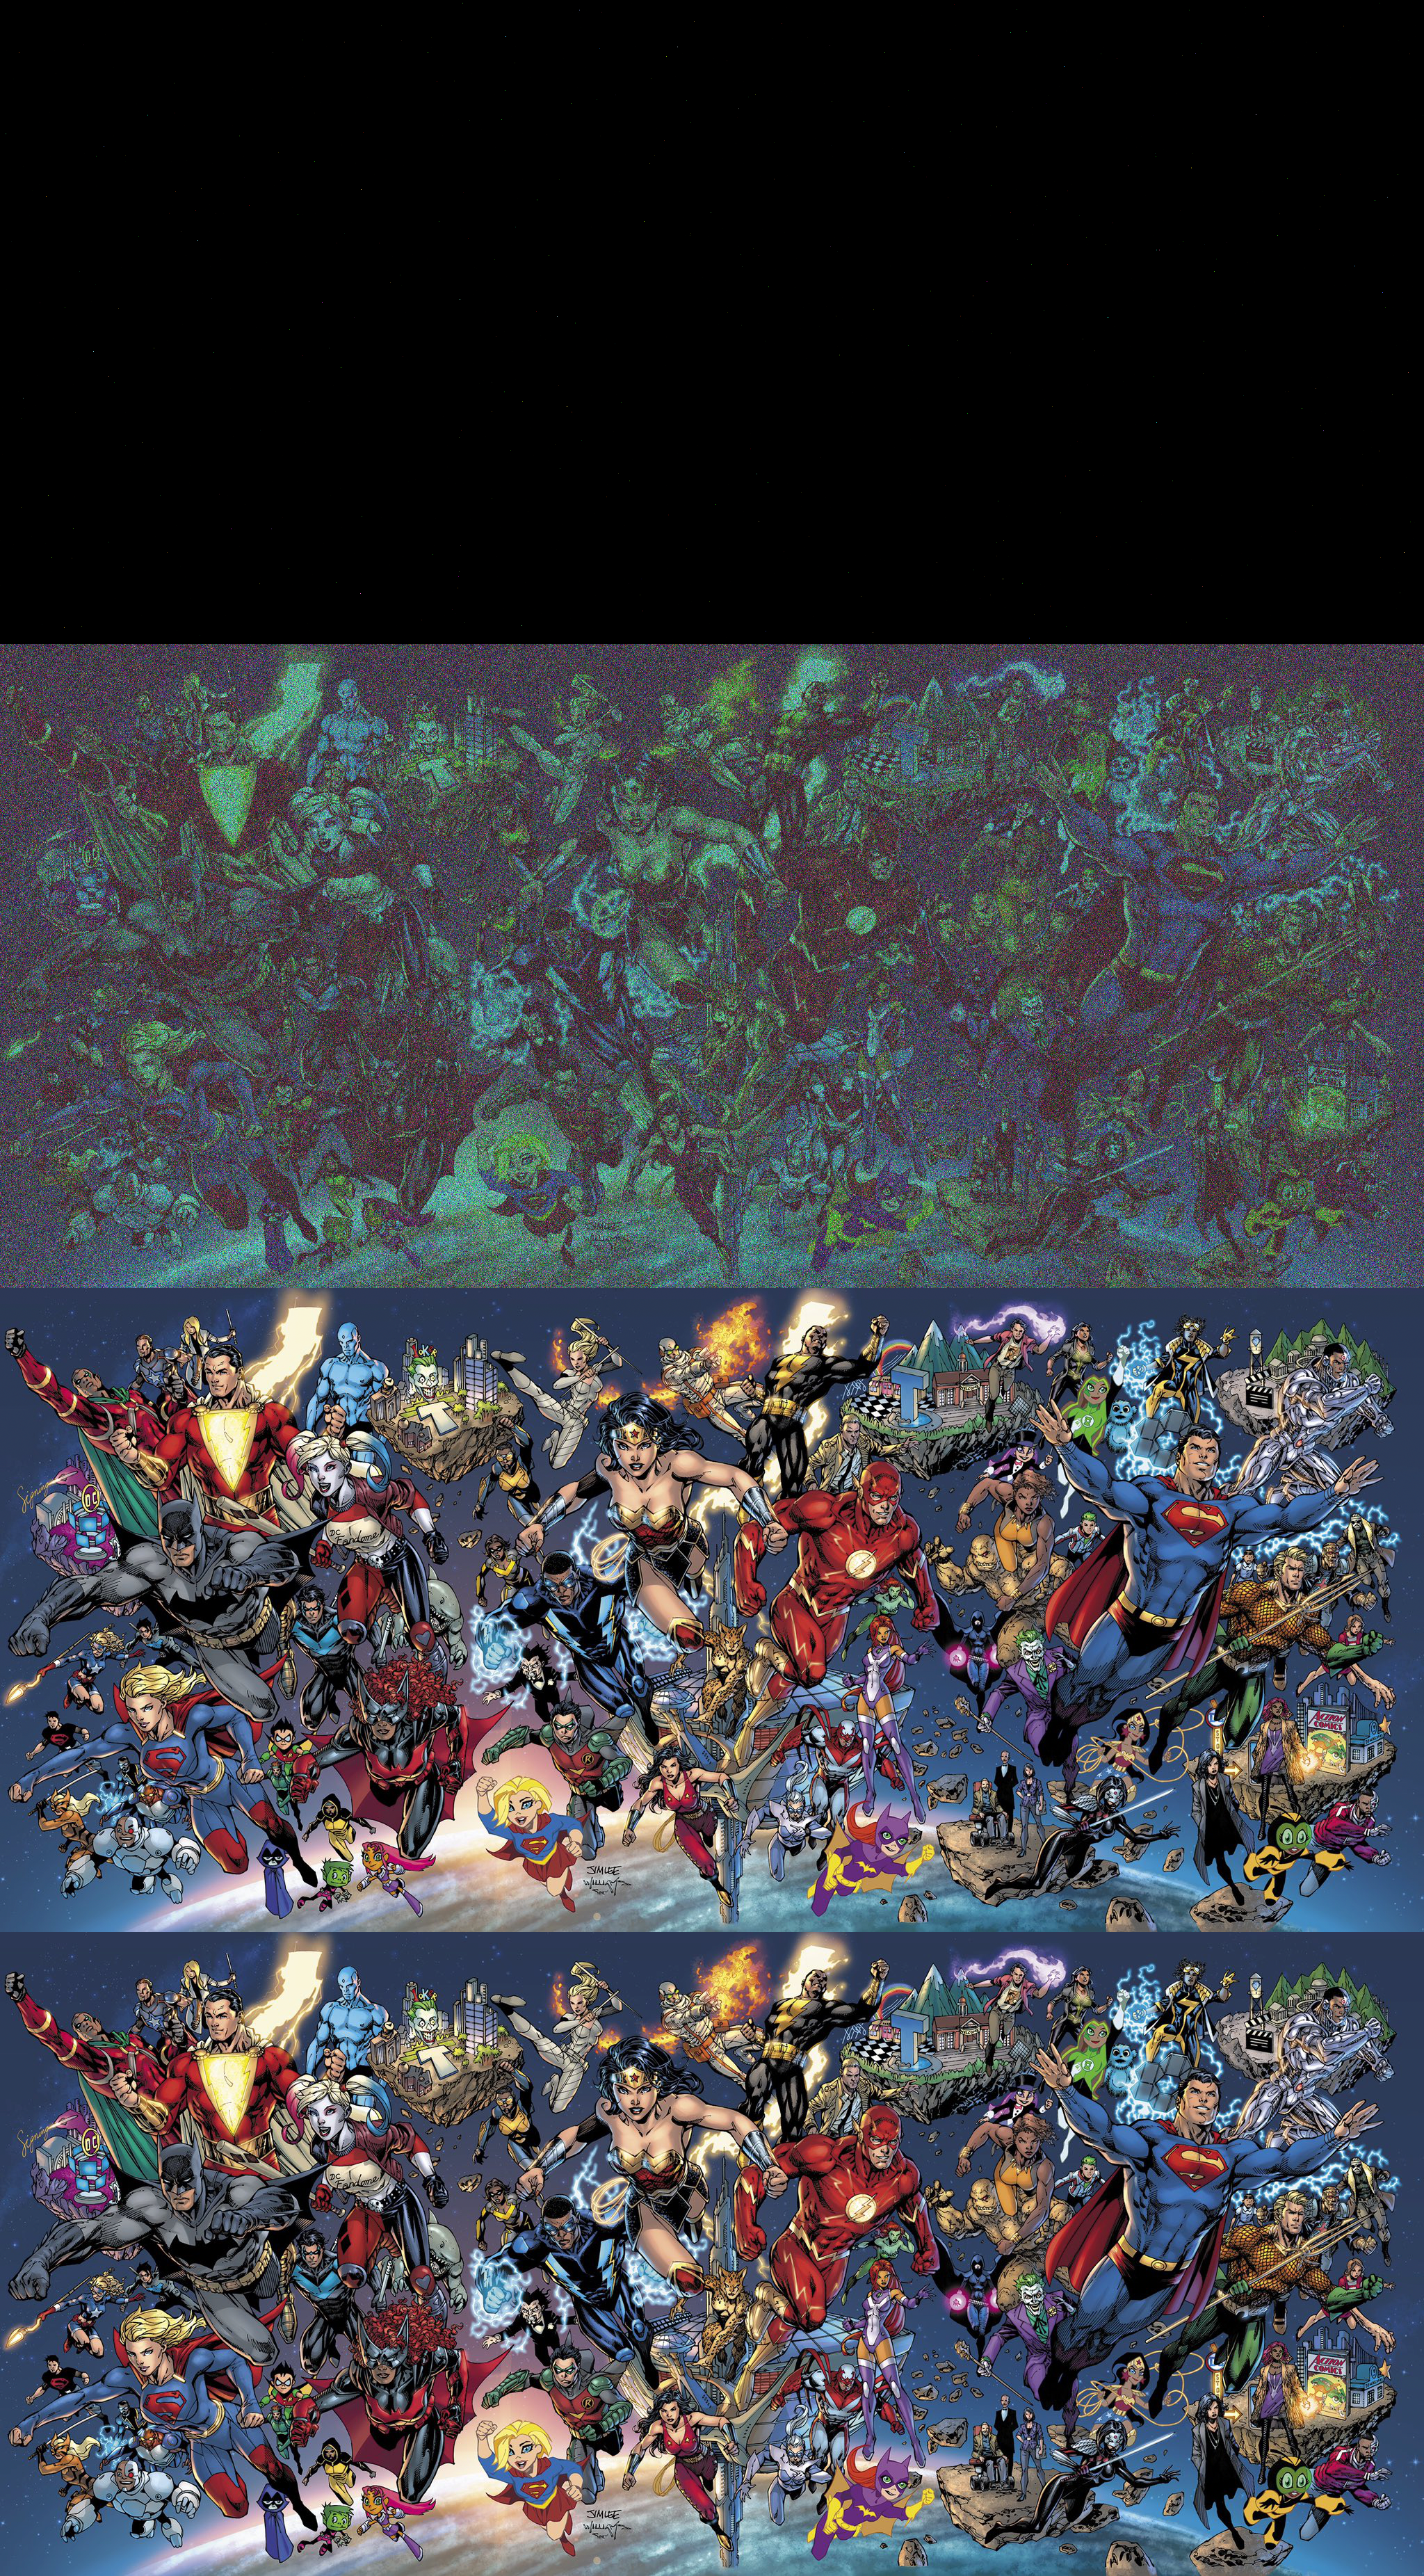
\includegraphics[width=0.90\textwidth]{./images/wf_dc/wf_dc_initial_emerging_final_oroginal.png}
    \caption{WF on DC\textregistered\space Universe Characters from Top to Buttom: After Initialization, 
	at Iteration $=121$, the Final Image, and the Original Image}
    \label{fig:wf_dc_initial_emerging_final_oroginal}
  \end{figure}
  \clearpage % End the page
}
 
% \cite{the_texbook_knuth}
\nocite{*}
\backmatter
% \glsxtrnewsymbol[description={inclusion signs}]{inclusion signs}{\ensuremath{\subset,\supset}}
\glsxtrnewsymbol[description={rational field}]{rational field}{\ensuremath{\mathbb{Q}}}
\glsxtrnewsymbol[description={least upper bound}]{least upper bound}{\ensuremath{\sup}}
\glsxtrnewsymbol[description={greatest lower bound}]{greatest lower bound}{\ensuremath{\inf}}

\glsxtrnewsymbol[description={null vector}]{null vector}{\ensuremath{\boldsymbol{0}}}
\glsxtrnewsymbol[description={inner product}]{inner product}{\ensuremath{\boldsymbol{x} \cdot \boldsymbol{y}}}
\glsxtrnewsymbol[description={elementwise absolute value of a multidimensional array $\boldsymbol{X}$} in the vector space $X$]{elementwise abs}{\ensuremath{\left| \boldsymbol{X}\right|_{e_X} }}\index{Product!Elementwise}
\glsxtrnewsymbol[description={elementwise/Hadamard product between two multidimensional array $\boldsymbol{X},\boldsymbol{Y}$}]{elementwise prod}{\ensuremath{\boldsymbol{X}\odot\boldsymbol{Y}}}\index{Product!Hadamard}
\glsxtrnewsymbol[description={sequence}]{sequence}{\ensuremath{\{x_n\}}}
\glsxtrnewsymbol[description={union}]{union}{\ensuremath{\bigcup,\cup}}
\glsxtrnewsymbol[description={intersection}]{intersection}{\ensuremath{\bigcap,\cap}}
\glsxtrnewsymbol[description={segment}]{segment}{\ensuremath{\left(a,b\right)}}
\glsxtrnewsymbol[description={interval}]{interval}{\ensuremath{\left[a,b\right]}}
\glsxtrnewsymbol[description={half intervals}]{half intervals}{\ensuremath{\left(a,b\right],\left[a,b\right)}}
\glsxtrnewsymbol[description={complement of $E$}]{complement of E}{\ensuremath{E^\mathsf{c}}}
\glsxtrnewsymbol[description={limit points of $E$}]{limit points of E}{\ensuremath{E^{'}}}
\glsxtrnewsymbol[description={closure of $E$}]{closure of E}{\ensuremath{\overline{E}}}
\glsxtrnewsymbol[description={limit}]{limit}{\ensuremath{\lim}}
\glsxtrnewsymbol[description={converges to}]{converges to}{\ensuremath{\to}}
\glsxtrnewsymbol[description={lim sup}]{lim sup}{\ensuremath{\lim \sup}}
\glsxtrnewsymbol[description={lim inf}]{lim inf}{\ensuremath{\lim \inf}}
\glsxtrnewsymbol[description={composition}]{composition}{\ensuremath{g \circ f}}
\glsxtrnewsymbol[description={right-hand limit}]{right-hand limit}{\ensuremath{f(x+)}}
\glsxtrnewsymbol[description={left-hand limit}]{left-hand limit}{\ensuremath{f(x-)}}
\glsxtrnewsymbol[description={derivatives}]{derivatives}{\ensuremath{f^{\prime}, \boldsymbol{f}(\boldsymbol{x})^{\prime}}}
\glsxtrnewsymbol[description={Riemann sums}]{Riemann sums}{\ensuremath{U(\boldsymbol{P},f),U(\boldsymbol{P},f,\alpha),L(\boldsymbol{P},f),L(\boldsymbol{P},f,\alpha)}}
\glsxtrnewsymbol[description={classes of Riemann (Stieltjes) integrable functionas}]{classes of Riemann (Stieltjes) integrable functionas}{\ensuremath{\mathcal{R},\mathcal{R}(\alpha)}}
\glsxtrnewsymbol[description={space of continiuous functions}]{space of continiuous functions}{\ensuremath{\mathcal{C}(X)}}
\glsxtrnewsymbol[description={norm}]{norm}{\ensuremath{\left|\left|\;\;\right|\right|}}
\glsxtrnewsymbol[description={exponential function}]{exponential function}{\ensuremath{\exp}}
\glsxtrnewsymbol[description={Dirichlet kernel}]{Dirichlet kernel}{\ensuremath{D_N}}
\glsxtrnewsymbol[description={gamma function}]{gamma function}{\ensuremath{\Gamma(x)}}

\glsxtrnewsymbol[description={spaces of linear transformation}]{spaces of linear transformation}{\ensuremath{L(X),L(X,Y)}}
\glsxtrnewsymbol[description={matrix}]{matrix}{\ensuremath{\left[\boldsymbol{A}\right]}}
\glsxtrnewsymbol[description={partial derivative}]{partial derivative}{\ensuremath{D_Jf}}
\glsxtrnewsymbol[description={gradient}]{gradient}{\ensuremath{\nabla f}}
\glsxtrnewsymbol[description={classes of differentiable functions}]{classes of differentiable functions}{\ensuremath{\mathcal{C}^\prime,\mathcal{C}^{\prime\prime}}}
\glsxtrnewsymbol[description={determinant}]{determinant}{\ensuremath{\det \left[\boldsymbol{A}\right]}}
\glsxtrnewsymbol[description={Jacobian}]{Jacobian_implicit}{\ensuremath{\boldsymbol{J}_f(\boldsymbol{x})}}
\glsxtrnewsymbol[description={Jacobian}]{Jacobian_explicit}{\ensuremath{\frac{\partial(y_1,\cdots,y_n)}{\partial(x_1,\cdots,x_n)}}}
\glsxtrnewsymbol[description={$k$-cell}]{k-cell}{\ensuremath{\mathbb{I}^k}}
\glsxtrnewsymbol[description={$k$-simplex}]{k-simplex}{\ensuremath{\mathbb{Q}^k}}
\glsxtrnewsymbol[description={basic $k$-form}]{basic k-form}{\ensuremath{d\boldsymbol{x}_{\boldsymbol{I}}}}
\glsxtrnewsymbol[description={multiplication symbol}]{multiplication symbol}{\ensuremath{^\wedge}}

\glsxtrnewsymbol[description={transform of $\omega$}]{transform of omega}{\ensuremath{\omega_{\boldsymbol{T}}}}
\glsxtrnewsymbol[description={boundary operator}]{boundary operator}{\ensuremath{\partial}}
\glsxtrnewsymbol[description={curl}]{curl}{\ensuremath{\nabla \times \boldsymbol{F}}}
\glsxtrnewsymbol[description={divergence}]{divergence}{\ensuremath{\nabla\cdot\boldsymbol{F}}}
\glsxtrnewsymbol[description={ring of elementary sets}]{ring of elementary sets}{\ensuremath{\mathcal{E}}}
\glsxtrnewsymbol[description={Lebesgue measure}]{Lebesgue measure}{\ensuremath{m}}
\glsxtrnewsymbol[description={measure}]{measure}{\ensuremath{\mu}}
\glsxtrnewsymbol[description={families of measurable sets}]{families of measurable sets}{\ensuremath{\mathcal{M}_F,\mathcal{M}}}
\glsxtrnewsymbol[description={positive(negative) part of $f$}]{posotove(negative) part of $f$}{\ensuremath{f^+,f^-}}
\glsxtrnewsymbol[description={characteristic function}]{characteristic function}{\ensuremath{K_{E}}}
\glsxtrnewsymbol[description={classes of Lebesgue-integrable functions}]{classes of Lebesgue-integrable functions}{\ensuremath{\mathcal{L},\mathcal{L}(\mu),\mathcal{L}^2,\mathcal{L}^2(\mu)}}


%%%%%%%%%%%%%%%%%%%%%%%%%%%%%%%%%%%%%%%%%%%%%%%%%%%%%%%%%%%%%%%%%%%%%%%%%%%%%%%%%%%%%%%%%%%%%%%%%%%%%%%%%%%%%%%%%%%%%%%
%%%%%%%%%%%%%%%%%%%%%%%%%%%%%%%%%%%%%%%%%%%%%%%%%%%%%%%%%%%%%%%%%%%%%%%%%%%%%%%%%%%%%%%%%%%%%%%%%%%%%%%%%%%%%%%%%%%%%%%
%%%%%%%%%%%%%%%%%%%%%%%%%%%%%%%%%%%%%%%%%%%%%%%%%%% Used Symbols %%%%%%%%%%%%%%%%%%%%%%%%%%%%%%%%%%%%%%%%%%%%%%%%%%%%%%
%%%%%%%%%%%%%%%%%%%%%%%%%%%%%%%%%%%%%%%%%%%%%%%%%%%%%%%%%%%%%%%%%%%%%%%%%%%%%%%%%%%%%%%%%%%%%%%%%%%%%%%%%%%%%%%%%%%%%%%
%%%%%%%%%%%%%%%%%%%%%%%%%%%%%%%%%%%%%%%%%%%%%%%%%%%%%%%%%%%%%%%%%%%%%%%%%%%%%%%%%%%%%%%%%%%%%%%%%%%%%%%%%%%%%%%%%%%%%%%
\glsxtrnewsymbol[description={inequality signs}]{inequality signs}{\ensuremath{<,\leq,>,\geq}}
\glsxtrnewsymbol[description={belongs to}]{in}{\ensuremath{\in}}  
\glsxtrnewsymbol[description={does not belong to}]{not in}{\ensuremath{\notin}}
\glsxtrnewsymbol[description={scalar product on the vector space $X$}]{scalar product}{\ensuremath{\left( \boldsymbol{\cdot} , \boldsymbol{\cdot} \right)_X}}
\glsxtrnewsymbol[description={the norm induced by the scalar product on the vector space $X$}]{induced norm}{\ensuremath{\left| \boldsymbol{\cdot} \right|_X}}
\glsxtrnewsymbol[description={absolute value/element-wise absolute value}]{absolute value/element-wise absolute value}{\ensuremath{\left| z \right|}}
\glsxtrnewsymbol[description={exponential}]{exponential}{\ensuremath{\exp}} 
\glsxtrnewsymbol[description={summation over $i$}]{summation over $i$}{\ensuremath{\sum_{i=p}^{i=q}a(i)}}



\glsxtrnewsymbol[description={real field}]{real field}{\ensuremath{\mathbb{R}}}
\glsxtrnewsymbol[description={complex field}]{complex field}{\ensuremath{\mathbb{C}}}
\glsxtrnewsymbol[description={euclidean $d$-space}]{euclidean $d$-space}{\ensuremath{\mathbb{R}^d}}
\glsxtrnewsymbol[description={complex $d$-space}]{complex $d$-space}{\ensuremath{\mathbb{C}^d}}

\glsxtrnewsymbol[description={infinities}]{infinities}{\ensuremath{+\infty,-\infty,\infty}}


\glsxtrnewsymbol[description={operator $\boldsymbol{A}$}]{operator A}{\ensuremath{\boldsymbol{A}}}
\glsxtrnewsymbol[description={adjoint operator of the operator $\boldsymbol{A}$}]{adjoint operator of the operator A}{\ensuremath{\boldsymbol{A}^*}}
\glsxtrnewsymbol[description={complex conjugate}]{complex conjugate}{\ensuremath{\overline{z}}}
\glsxtrnewsymbol[description={real part}]{real part}{\ensuremath{\operatorname{Re}(z)}}
\glsxtrnewsymbol[description={imaginary part}]{imaginary part}{\ensuremath{\operatorname{Im}(z)}}
\glsxtrnewsymbol[description={summation sign}]{summation sign}{\ensuremath{\sum}}

\glsxtrnewsymbol[description={standard cartesian basis}]{standard cartesian basis}{\ensuremath{\{\boldsymbol{e}_1,\cdots,\boldsymbol{e}_n\}}}
\glsxtrnewsymbol[description={general $1$-$d$ basis}]{general $1$-$d$ basis}{\ensuremath{\{\boldsymbol{g}^1,\cdots,\boldsymbol{g}^n\}}}
\glsxtrnewsymbol[description={general $2$-$d$ basis}]{general $2$-$d$ basis}{\ensuremath{\left\{\boldsymbol{g}^{i,j}\right\}_{\substack{i=1,\ldots,m\\ j=1,\ldots,n}}}}
\glsxtrnewsymbol[description={differentiation operator}]{differentiation operator}{\ensuremath{\mathrm{d}}}
% \glsxtrnewsymbol[description={differentiation operator multidimensional for }]{differentiation operator multidimensional}{\ensuremath{\mathrm{d}}}
\printunsrtglossary[type=symbols,style=long,title=Acronyms and List of Special Symbols]
% \bibliographystyle{siam}
\printindex
\printbibliography

\end{document}